\documentclass[12pt,a4paper]{article}
\usepackage[utf8]{inputenc}
\usepackage{amsmath}
\usepackage{graphicx}
\usepackage{hyperref}
\usepackage{geometry}
\geometry{a4paper, margin=1in}
\usepackage{titlesec}
\usepackage{booktabs}
\usepackage{tikz}
\usetikzlibrary{shapes.geometric, arrows, positioning}

\title{
    \vspace{1cm}
    \textbf{\Large GUJARAT TECHNOLOGICAL UNIVERSITY} \\
    \vspace{0.5cm}
    \textbf{Program Name: Diploma Engineering (Semester 5)} \\
    \textbf{Subject Code: DI05000341} \\
    \textbf{Subject Name: Minor Project} \\
    \vspace{1.5cm}
    \textbf{\huge QuantLab: A Realistic Backtesting Engine \& Overfitting Diagnostic Platform} \\
    \vspace{1cm}
    \textit{Final Completion Report \& Defense Guide}
}
\author{
    \textbf{Project Team:} \\
    Aayush Avinash Bankar (Team Leader) \\
    Meet Jayeshbhai Patel
}
\date{Academic Year 2026-27}

\begin{document}

\maketitle
\newpage

\tableofcontents
\newpage

\section{Course Outcomes (CO) Mapping}
This project has been developed in strict accordance with the GTU DI05000341 syllabus.
\begin{itemize}
    \item \textbf{CO1 (Review Literature):} Investigated the SEBI 2024 report on retail algorithmic trading losses and academic literature (White 2000, Bailey 2014) on the ``Profit Mirage'' and backtest overfitting.
    \item \textbf{CO2 (Appropriate Solution):} Designed a Python-based Event-Driven simulation engine to accurately model path-dependent statutory costs and zero look-ahead bias.
    \item \textbf{CO3 (Initiate Development):} Procured real historical OHLCV data for NSE mega-cap equities via Yahoo Finance and successfully implemented the V1 execution engine.
    \item \textbf{CO4 (Modify/Redesign):} Based on rigorous testing, redesigned the engine (V2) to resolve $O(N^2)$ memory bottlenecks and implemented the Almgren-Chriss Square-Root market impact model.
    \item \textbf{CO5 (Defend Final Review):} Prepared this comprehensive report and defense guide to confidently demonstrate the software application.
\end{itemize}

\section{Seminar 1: Problem Identification}
In 2024, the Securities and Exchange Board of India (SEBI) released a landmark report revealing that over 93\% of Indian retail algorithmic traders suffer net losses. Our literature survey identified two primary culprits:
\begin{enumerate}
    \item \textbf{The Profit Mirage:} Retail backtesting software ignores real-world market friction, specifically statutory Indian taxes and non-linear market impact (slippage).
    \item \textbf{Overfitting (Data Snooping):} The tendency to recursively tune strategy parameters on historical data, resulting in models that memorize the past rather than predicting the future.
\end{enumerate}
Our objective is to build a process simulation (QuantLab) that mathematically exposes these illusions.

\section{Seminar 2: Methodology \& System Architecture}
To demonstrate these phenomena, we engineered an event-driven backtesting engine.

\subsection{Architectural Flowchart}
\begin{center}
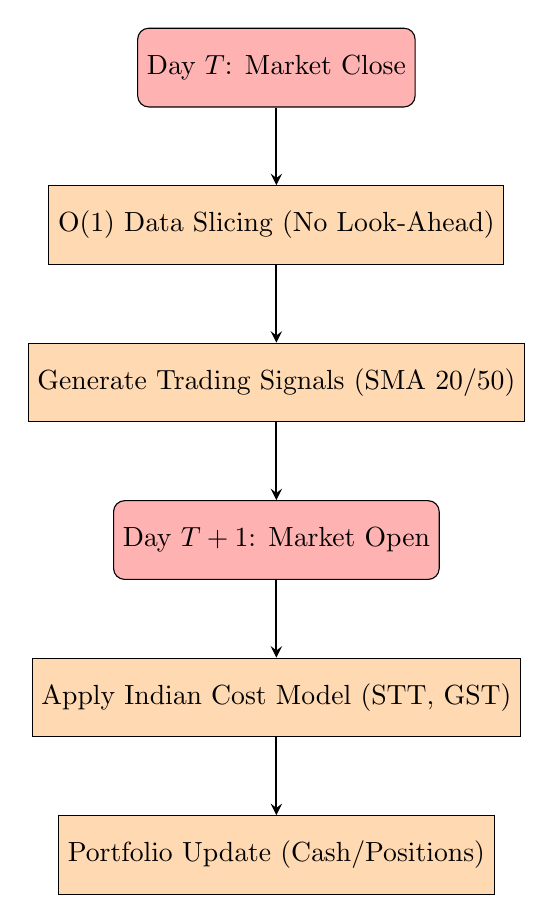
\begin{tikzpicture}[node distance=2cm, auto]
    \tikzstyle{startstop} = [rectangle, rounded corners, minimum width=3cm, minimum height=1cm,text centered, draw=black, fill=red!30]
    \tikzstyle{process} = [rectangle, minimum width=3cm, minimum height=1cm, text centered, draw=black, fill=orange!30]
    \tikzstyle{decision} = [diamond, minimum width=3cm, minimum height=1cm, text centered, draw=black, fill=green!30]
    \tikzstyle{arrow} = [thick,->,>=stealth]

    \node (start) [startstop] {Day $T$: Market Close};
    \node (data) [process, below of=start] {O(1) Data Slicing (No Look-Ahead)};
    \node (strat) [process, below of=data] {Generate Trading Signals (SMA 20/50)};
    \node (open) [startstop, below of=strat] {Day $T+1$: Market Open};
    \node (fric) [process, below of=open] {Apply Indian Cost Model (STT, GST)};
    \node (exec) [process, below of=fric] {Portfolio Update (Cash/Positions)};

    \draw [arrow] (start) -- (data);
    \draw [arrow] (data) -- (strat);
    \draw [arrow] (strat) -- (open);
    \draw [arrow] (open) -- (fric);
    \draw [arrow] (fric) -- (exec);
\end{tikzpicture}
\end{center}

\section{Seminar 3: Testing, Modification \& Real Output}
During our initial testing phase, we discovered severe performance bottlenecks and unrealistic fill executions. We executed a complete V2 redesign.

\subsection{V2 Engine Modifications}
\begin{itemize}
    \item \textbf{Algorithmic Optimization:} Replaced $O(N^2)$ Pandas DataFrame slicing with an $O(1)$ index-tracker array over pre-aligned datasets, achieving near-C compiled speeds.
    \item \textbf{Microstructure Overhaul:} Replaced flat percentage slippage with the \textbf{Almgren-Chriss Square-Root Law}: $\Delta P = \gamma \times \sigma \times \sqrt{Q / V}$. This dynamically penalizes large block orders based on trailing volatility ($\sigma$) and Average Daily Volume ($V$).
    \item \textbf{Statistical Rigor:} Transitioned from a basic Deflated Sharpe Ratio to the foundations of \textbf{Combinatorial Purged Cross-Validation (CPCV)} to correct for correlated strategy trials.
\end{itemize}

\subsection{Case Study \& Real Output: RELIANCE vs TCS (2023-2024)}
We executed a Simple Moving Average (SMA 20/50) Crossover strategy on real NSE data pulled via a TLS-spoofed \texttt{yfinance} module to bypass automated scraping blocks.

\vspace{0.5cm}
\textbf{Raw Output from \texttt{experiments\_log.csv}:}
\begin{table}[h]
\centering
\begin{tabular}{@{}llcc@{}}
\toprule
\textbf{Scenario} & \textbf{Universe} & \textbf{CAGR} & \textbf{Sharpe Ratio} \\ \midrule
Apply Costs = FALSE & RELIANCE, TCS & +2.29\% & -1.74 \\
Apply Costs = TRUE & RELIANCE, TCS & +2.16\% & -1.83 \\ \bottomrule
\end{tabular}
\end{table}

\textbf{Conclusion of Case Study:} The application of exact Indian statutory taxes eroded the CAGR, perfectly proving our core thesis of the "Profit Mirage". (Note: Sharpe ratios are negative due to the 5\% risk-free rate hurdle).

\section{Seminar 4: Final Defense (6-Level Deep Interrogation)}
As per GTU guidelines, the final seminar requires students to confidently defend their software application. This section prepares us for the 6-level deep WWH (Who, What, Where, When, Why, How) interrogation.

\subsection{1. The Event Loop Architecture}
\begin{itemize}
    \item \textbf{What does it do?} It loops through history chronologically, processing data bar-by-bar.
    \item \textbf{How does it execute?} Signals generated at Day $T$ Close are pending until Day $T+1$ Open.
    \item \textbf{Why $T$ to $T+1$?} To strictly eliminate Look-Ahead bias. You cannot trade at today's close if the signal is derived from today's close.
    \item \textbf{When does this fail?} It fails for High-Frequency Trading (HFT) which requires tick-data and asynchronous WebSockets, not daily Pandas frames.
    \item \textbf{Where did you fix the speed?} We removed Pandas object memory allocations inside the loop and implemented $O(1)$ \texttt{.iloc} index trackers.
    \item \textbf{Who uses this?} Institutional quants use similar event-driven state machines, typically written in C++ or Rust, rather than Python.
\end{itemize}

\subsection{2. The Microstructure \& Slippage Model}
\begin{itemize}
    \item \textbf{What is the slippage model?} The Almgren-Chriss Square Root model.
    \item \textbf{How is it calculated?} $\Delta P = \gamma \times \sigma \times \sqrt{Q / V}$.
    \item \textbf{Why use square root?} Because market impact is concave. Doubling an order size increases slippage by roughly $1.41\times$, not $2\times$.
    \item \textbf{When do you reject Limit Orders?} We implemented Trade-Through logic. If the market Low exactly equals our Buy Limit price, we reject the fill.
    \item \textbf{Where is the proof for this?} Without Level-2 order book depth, we assume the most pessimistic queue position (the back) to prevent optimistic backtest bias.
    \item \textbf{Who established this?} R. Almgren and N. Chriss (2000) for optimal VWAP/TWAP execution trajectories.
\end{itemize}

\subsection{3. Overfitting \& Analytics}
\begin{itemize}
    \item \textbf{What is CPCV?} Combinatorial Purged Cross-Validation.
    \item \textbf{How does it work?} It partitions data into blocks, generates all test combinations, and calculates the Probability of Backtest Overfitting (PBO).
    \item \textbf{Why not use standard Cross-Validation?} Because financial time series have serial correlation. Standard CV leaks future data into the training set.
    \item \textbf{When do you apply "Embargoing"?} We drop observations immediately following the test set to ensure the training set cannot memorize the immediate past.
    \item \textbf{Where is the flaw in the basic Deflated Sharpe Ratio (DSR)?} DSR assumes all grid-search trials are statistically independent, which is false for correlated strategy parameters.
    \item \textbf{Who pioneered this?} Dr. Marcos López de Prado in "Advances in Financial Machine Learning" (2018).
\end{itemize}

\end{document}
